%; whizzy chapter$B!!(B-dvi
% -initex iniptex -latex platex -format platex -bibtex jbibtex -fmt fmt
% $B0J>e(B whizzytex $B$r;HMQ$9$k>l9g$N@_Dj!#(B

%     Tokyo Debian Meeting resources
%     Copyright (C) 2012 Junichi Uekawa
%     Copyright (C) 2011 Nobuhiro Iwamatsu

%     This program is free software; you can redistribute it and/or modify
%     it under the terms of the GNU General Public License as published by
%     the Free Software Foundation; either version 2 of the License, or
%     (at your option) any later version.

%     This program is distributed in the hope that it will be useful,
%     but WITHOUT ANY WARRANTY; without even the implied warranty of
%     MERCHANTABILITY or FITNESS FOR A PARTICULAR PURPOSE.  See the
%     GNU General Public License for more details.

%     You should have received a copy of the GNU General Public License
%     along with this program; if not, write to the Free Software
%     Foundation, Inc., 51 Franklin St, Fifth Floor, Boston, MA  02110-1301 USA

%  preview (shell-command (concat "evince " (replace-regexp-in-string "tex$" "pdf"(buffer-file-name)) "&"))
% $B2hA|%U%!%$%k$r=hM}$9$k$?$a$K$O(Bebb$B$rMxMQ$7$F(Bboundingbox$B$r:n@.!#(B
%(shell-command "cd image201201; ebb *.png")

%%$B$3$3$+$i%X%C%@3+;O!#(B

\documentclass[mingoth,a4paper]{jsarticle}
\usepackage{monthlyreport}

% $BF|IU$rDj5A$9$k!"Kh7nJQ$o$j$^$9!#(B
\newcommand{\debmtgyear}{2013}
\newcommand{\debmtgmonth}{3}
\newcommand{\debmtgdate}{16}
% started from zero:
% (let ((year 2013) (month 1)) (+ (* (- year 2005) 12) month -1))
\newcommand{\debmtgnumber}{96}

\begin{document}

\begin{titlepage}
\thispagestyle{empty}
% $B%?%$%H%k%Z!<%8(B:$BJT=8I,MW$JItJ,$O:G=i$N%^%/%m$KHt$P$9$3$H(B

\vspace*{-2cm}
$BBh(B\debmtgnumber{}$B2s(B $BEl5~%(%j%"(B Debian $BJY6/2q;qNA(B\\
\hspace*{-2cm}

\includegraphics{image2012-natsu/dotdeb.pdf}\\
\hfill{}\debmtgyear{}$BG/(B\debmtgmonth{}$B7n(B\debmtgdate{}$BF|(B

% $B$3$3$O%"%C%W%G!<%H$9$k$3$H(B
% $BA43QJ8;z$K$7$J$$$H%U%)%s%H$N%5%$%:$,9g$o$J$$$N$GCm0U(B
\rotatebox{10}{\fontsize{32}{32} {\gt $BFC=8#1!'(B $B#g#d#b!!#p#y#t#h#o#n3HD%(B}}

\rotatebox{10}{\fontsize{32}{32} {\gt $BFC=8#2!'(B $B#s#a#m#b#a#4(B}}

\vspace*{-2cm}
\hfill{}
\includegraphics[height=6cm]{image200502/openlogo-nd.eps}
\end{titlepage}

\dancersection{Introduction}{$B>e@n(B $B=c0l(B}

\begin{multicols}{2}
 

 $B:#7n$N(BDebian$BJY6/2q$X$h$&$3$=!#$3$l$+$i(BDebian$B$N@$3&$K$"$7$rF'$_F~$l$k$H(B
 $B$$$&J}$b!"$9$G$K$I$C$W$j$H$D$+$C$F$$$k$H$$$&J}$b!"7n$K0l2s(BDebian$B$K$D$$(B
 $B$F8l$j$^$;$s$+!)(B

 Debian$BJY6/2q$NL\E*$O2<5-$G$9!#(B

 \begin{itemize}
 \item \underline{Debian Developer} ($B3+H/<T(B)$B$N0i@.!#(B
 \item $BF|K\8l$G$N!V(B\underline{$B3+H/$K4X$9$k>pJs(B}$B!W$r@0M}$7$F$^$H$a!"%"%C%W%G!<%H$9$k!#(B
 \item \underline{$B>l(B}$B$NDs6!!#(B
 \begin{itemize}
  \item $BIaCJ$P$i$P$i$J>l=j$K$$$k?M!9$,(B face-to-face $B$G=P2q$($k>l$rDs6!(B
	$B$9$k!#(B
  \item Debian $B$N$?$a$K$J$k$3$H$r8l$k>l$rDs6!$9$k!#(B
  \item Debian$B$K$D$$$F8l$k>l$rDs6!$9$k!#(B
 \end{itemize}
 \end{itemize}		

 Debian$B$NJY6/2q$H$$$&$3$H$G5f6KE*$K$O;22C<TA40w$,(BDebian Package$B$r$,$j$,$j(B
 $B$H:n$k%9!<%Q!<%O%C%+!<$K$J$C$?;Q$rLQA[$7$F$$$^$9!#>pJs$N6&M-!&3hMQ$rDL$7(B
 $B$F(B Debian$B$N:#8e$NG=F0E*$JE83+$X$NEZBf$H$7$F!"!V>l!W$H$7$F$N6u4V$rDs6!$9(B
 $B$k$N$,L\E*$G$9!#(B

\end{multicols}

\newpage

\begin{minipage}[b]{0.2\hsize}
 \definecolor{titleback}{gray}{0.9}
 \colorbox{titleback}{\rotatebox{90}{\fontsize{80}{80} {\gt $B%G%S%"%sJY6/2q(B} }}
\end{minipage}
\begin{minipage}[b]{0.8\hsize}
\hrule
\vspace{2mm}
\hrule
\begin{multicols}{2}
\tableofcontents
\end{multicols}
\vspace{2mm}
\hrule
\end{minipage}

\dancersection{$B;vA02]Bj(B}{$BL$Dj(B}

$B:#2s$N;vA02]Bj$O0J2<$G$9(B:
\begin{enumerate}
 \item $BL$Dj(B
\end{enumerate}
$B$3$N2]Bj$KBP$7$FDs=P$$$?$@$$$?FbMF$O0J2<$G$9!#(B

\dancersection{Debian Trivia Quiz}{$BL$Dj(B}

$B$H$3$m$G!"$_$J$5$s(B Debian $B4XO"$NOCBj$K$*$$$D$$$F$$$^$9$+!)(BDebian$B4XO"$NOC(B
$BBj$O%a!<%j%s%0%j%9%H$r$h$s$G$$$k$HDI@W$G$-$^$9!#$?$@$h$s$G$$$k$@$1$G$O$O(B
$B$j$"$$$,$J$$$N$G!"M}2rEY$N%F%9%H$r$7$^$9!#FC$K0l?M$@$1$G$O0UL#$,$o$+$i$J(B
$B$$$H$3$m$b$"$k$+$bCN$l$^$;$s!#$_$s$J$G0l=o$KFI$s$G$_$^$7$g$&!#(B

\dancersection{$B:G6a$N(BDebian$B4XO"$N%_!<%F%#%s%0Js9p(B}{$BL$Dj(B}
\subsection{OSC$BEl5~Js9p(B}
% (query-replace-regexp "<.*?>" "")
% (query-replace-regexp "^[	 ]\+" "")

$B#2#0#1#3G/#27n$N(BOSC$BEl5~$OL@@1Bg3X$G3+:E$5$l$^$7$?!#(B
$B%;%_%J!<C4Ev$OLnEg$5$s(B
$BE8<(C4Ev$O(Bkoedoyoshida$B$5$s(B
dictoss$B$5$s!"$d$^$M$5$s$,6(NO$7$^$7$?!#(B
$B>\:Y$O8e$[$I(B

%-------------------------------------------------------------------------------
\dancersection{gdb python$B3HD%$=$N(B1}{$BLnEg(B $B5.1Q(B}
%-------------------------------------------------------------------------------
\index{gdb-python$B$+$/$A$g$&(B@gdb-python$B3HD%(B}
\subsection{$B$O$8$a$K(B}

 Debian$B%Q%C%1!<%8$N%P%$%J%j$N%P%0DY$7$r9T$&;~!"(Bgdb$B$J$I$N%G%P%C%,$r;H$C$F%G%P%C%0$r(B
$B$9$k;v$bB?$$$+$H;W$$$^$9!#$7$+$7$J$,$i!"%W%m%0%i%`$N9=B$$,Bg5,LO(B/$BJ#;($K$J$C$F$/$k$H!"(B
$B%G%P%C%0:n6H$bBgJQ$K$J$C$F$$$-$^$9!#$^$?!"%W%m%0%i%`$K$D$$$F$b!"(B
$BCj>]2=$,7c$7$/9T$o$l$F$$$k$H!"%G%P%C%,L5$7$K$O2r@O$,Hs>o$K:$Fq$+$H;W$$$^$9!#(B

 gdb$B$O(Bv7.0$B$+$i(Bpython$B3HD%$,Ek:\$5$l$F$*$j!"(Bgdb$B$r(Bpython$B%9%/%j%W%H$GA`$k(B
$B;v$,$G$-$^$9!#$3$A$i$rMxMQ$9$k;v$K$h$j!"?M<j$G$O!"9)?t$+$+$j$9$.$G$J$+$J$+(B
$B?J$^$J$+$C$?%G%P%C%0$b2DG=$K$J$C$F$$$/$H;W$$$^$9!#(B

 $B:#2s$O!"(Bgdb$B$N(Bpython$B3HD%$N0lIt$r@bL@$7!":G8e$O(BC$B8@8l$G:n$i$l$?(B
$B%W%m%0%i%`$N<B9T%H%l!<%9$r<B:]$K(Bpython$B3HD%5!G=$rMQ$$$F!"<hF@$7$F$_$k(B
$B$H$3$m$^$G$d$C$F$_$^$9!#(B

\subsection{Debian sid$B$N(Bgdb python$B3HD%$N4pK\>pJs(B}

 debian sid$B$K4^$^$l$F$$$k(Bgdb$B$O:G=i$+$i(Bpython$B3HD%$,M-8z$K$7$F$"$k$h$&$G$9!#(B
$BI=(B\ref{tab:gdb-python-basic-info}$B$K4pK\>pJs$r:\$;$^$9!#(B

\begin{table}[ht]
\begin{center}
\small
\begin{tabular}{|l|l|l|}
\hline
$B9`HV(B & $B9`L\(B & $BCM(B \\
\hline
1 & gdb$B%P!<%8%g%s(B & 7.4.1 \\
2 & python$B%P!<%8%g%s(B & 2.7.3 \\
3 & python$B%5!<%A%Q%9(B & /usr/share/gdb/python,/usr/lib/python2.7$B0J2<(B \\
\hline
\end{tabular}
\caption{Debian sid$B4D6-$K4^$^$l$k(Bgdb$B$H(Bpython$B$N4pK\>pJs(B}
\label{tab:gdb-python-basic-info}
\end{center}
\end{table}

 $B:#2s$O(Bdebian sid amd64$B4D6-$G%F%9%H$7$?7k2L$r85$K@bL@$r9T$$$^$9!#(B

\subsection{python$B3HD%$r4J0WE*$KF0$+$7$F$_$k(B}

 gdb$B$h$j(Bpython$B8@8l$r4J0WE*$K8F$S=P$9>l9g!"(Bgdb$B$N%3%^%s%I%i%$%s$+$i@\F,<-$H$7$F(B
python$B$r$D$1$F5/F0$7$^$9!#$^$?!"(Bgdb$B%3%^%s%I%i%$%s$+$i(B
python$B$N$_$r;XDj$9$k$H!"(BCtrl+d$B$r2!2<$9$k$^$G!"J#?t$N(Bpython$B9=J8$r(B
$B;XDj$G$-$^$9!#(B($B$J$*!"(BCtrl+d$B$r2!2<$9$k$H!"(Bgdb$B$N%3%^%s%I%i%$%s$KI|5"$9$k(B
$B$HF1;~$KF~NO$7$?J#?t$N(Bpython$B9=J8$,0lEY$KI>2A$5$l$^$9!K(B

 $B$J$*!"(Bpython$B$G0lEYDj5A$7$?JQ?t$J$I$O(Bgdb$B$r=*N;$9$k$^$G2?EY$G$b(B
$B;2>H$G$-$^$9!#(B

\begin{commandline}
$ gdb 
GNU gdb (GDB) 7.4.1-debian
Copyright (C) 2012 Free Software Foundation, Inc.
...$BCfN,(B...
For bug reporting instructions, please see:
<http://www.gnu.org/software/gdb/bugs/>.
(gdb) python print "hello world"
hello world
(gdb) python a=[1,2,3,4]
(gdb) python print a
[1, 2, 3, 4]
(gdb) python a.append(5)
(gdb) python print a
[1, 2, 3, 4, 5]
(gdb) python
>import sys
>print sys.path
>print sys.version_info
>$B$3$3$G(BCtrl+d
['/usr/share/gdb/python', '/usr/lib/python2.7',
  '/usr/lib/python2.7/plat-linux2', '/usr/lib/python2.7/lib-tk',
  '/usr/lib/python2.7/lib-old', '/usr/lib/python2.7/lib-dynload',
  '/usr/local/lib/python2.7/dist-packages',
  '/usr/lib/python2.7/dist-packages',
  '/usr/lib/python2.7/dist-packages/PIL',
  '/usr/lib/python2.7/dist-packages/gst-0.10',
  '/usr/lib/python2.7/dist-packages/gtk-2.0',
  '/usr/lib/pymodules/python2.7']
sys.version_info(major=2, minor=7, micro=3, releaselevel='final', serial=0)
\end{commandline}
% $ 
\subsection{gdb$B$N(Bpython$B3HD%$N9=B$(B}

$B!!(Bgdb$B$N(Bpython$B3HD%$O?^(B\ref{fig:python-internal-schema}$B$N$h$&$J9=B$$H$J$C$F$$$^$9!#(B

\begin{figure}[h]
\begin{center}
 \includegraphics[width=0.8\hsize]{image201301/gdb-python/gdb-python-internal-schema.eps}
 \caption{gdb$B$H(Bpython$B3HD%$N9=B$(B}
 \label{fig:python-internal-schema}
\end{center}
\end{figure}

\subsection{module gdb$B$N%^%K%e%"%k(B}

 gdb$BK\BN$K(Bmodule gdb$B$,<BAu$5$l$F$$$k$?$a!"(Bmodule gdb$B$N(B
python$B%I%-%e%a%s%H$K$D$$$F$O!"(Bgdb$B>e$G(Bpython$B$+$i(Bhelp(gdb)$B$r8F$S=P$9I,MW(B
$B$,$"$j$^$9!#(B

 $B0J2<$KFI$_J}$r<($7$^$9!#$J$*!"0J9_!"(B(gdb)$B$O(Bgdb$B$N%W%m%s%W%H$r<($7$^$9!#(B

\begin{commandline}
(gdb) python help(gdb)
Help on package gdb:

NAME
    gdb

FILE
    (built-in)

PACKAGE CONTENTS
    command (package)
    printing
    prompt
    types

...$BCfN,(B...
\end{commandline}

 $B$^$?!"(Bgdb$B$N(Bpython$B3HD%$K$D$$$F$N$5$i$K>\$7$$@bL@$O!"(Binfo gdb$B$K$F(B
Extending GDB$B"*(Bpython$B$N9`L\$+$i;2>H$G$-$^$9!#(B

\subsection{module gdb$B$KDj5A$5$l$F$$$k%*%V%8%'%/%H72(B}

 $B?^(B\ref{fig:python-class-schema-1}$B!A?^(B\ref{fig:python-class-schema-2}$B$K!"(B
module gdb$B$KDj5A$5$l$F$$$k%*%V%8%'%/%H72$N(Bclass$B?^$r:\$;$^$9!#(B

 gdb$B3HD%MQ$N(Bpython$B%9%/%j%W%H$r5-:\$9$k>l9g!"$3$l$i%*%V%8%'%/%H$rJ;MQ$7$F(B
gdb$B$H$N%G!<%?$N$d$j$H$j!"$"$k$$$O!"A`:n$r9T$$$^$9!#(B

\begin{figure}[h]
\begin{center}
 \includegraphics[width=0.8\hsize]{image201301/gdb-python/gdb-python-class-schema-1.eps}
 \caption{module gdb$B$N(Bclass$B?^(B($B$=$N(B1)}
 \label{fig:python-class-schema-1}
\end{center}
\end{figure}

\begin{figure}[h]
\begin{center}
 \includegraphics[width=0.8\hsize]{image201301/gdb-python/gdb-python-class-schema-2.eps}
 \caption{module gdb$B$N(Bclass$B?^(B($B$=$N(B2)}
 \label{fig:python-class-schema-2}
\end{center}
\end{figure}

\newpage

\subsection{gdb$B$N%3%^%s%I$rA}$d$7$F$_$k(B}

 gdb$B$N(Bpython$B3HD%$O=@Fp$J5!G=$r;}$D$?$a!"$$$m$$$m$J;H$$J}$,$G$-$^$9!#(B
$B$3$3$G$O!";n$7$K(Bgdb$B$N%3%^%s%I$rA}$d$7$F$_$^$9!#(B

$B!!(Bgdb$B$N%3%^%s%I$r(Bpython$B$+$iA}$d$9$K$O!"(Bgdb.command$B%/%i%9$r7Q>5$7$?%/%i%9$r(B
$BMQ0U$7!"(Bgdb.command.\_\_init\_\_()$B$K$F%3%^%s%IL>$H6&$KEPO?$9$k;v$K$h$j9T$$$^$9!#(B

$B!!(Binfo gdb$B$N(BExtending GDB$B"*(BPython$B"*(BPython API$B"*(BCommands In Python$B$K(B
$B5-:\$5$l$F$$$kJ}K!$r;n$7$F!"(Bhello-world$B%3%^%s%I$rEPO?$7$F$_$^$9!#(B

\begin{commandline}
-----hello.py$B$NCf?H$3$3$+$i(B-----
# -*- coding: utf-8 -*-
# coding:utf-8
import gdb
class HelloWorld (gdb.Command):
  """ Greet the whole world """
  def __init__ (self):
     super(HelloWorld, self).__init__ ("hello-world",gdb.COMMAND_OBSCURE)

  def invoke (self,arg, from_tty):
     print "Hello, World! arg=["+str(arg)+"]"

HelloWorld()
-----hello.py$B$NCf?H$3$3$^$G(B-----
\end{commandline}

 $BDI2C$7$?%3%^%s%I$K$D$$$F$$$m$$$m<B9T$7$F$_$^$9!#(B

\begin{commandline}
(gdb) source hello.py
(gdb) hello-[$B$3$3$G(BTAB$B$r2!$9$HJd40$5$l$k(B]
(gdb) hello-world foo,bar,com
Hello, World! arg=[foo,bar,com]
(gdb) help obscure
Obscure features.

List of commands:

...$BCfN,(B...
hello-world --  Greet the whole world 
...$BCfN,(B...
\end{commandline}

$B!!%3%^%s%I(B hello-world$B$,DI2C$5$l$F$$$^$9!#$^$?!"0z?t$O(Binvoke()$B$N(Barg$B$KJ8;zNs$H$7$F(B
$B$^$H$a$FF~$j$^$9!#$^$?!"%3%^%s%I%+%F%4%j$N(BOBSCURE$B$KEPO?$5$l$F$$$k;v$,(Bhelp obscure
$B$K$FH=$j$^$9!#(B

\subsection{$B:n$C$?(Bpython$B%9%/%j%W%H$r<+F0$GFI$_9~$^$;$k$K$O(B}

 $B$H$3$m$G!"(Bgdb$B$N(Bpython$B3HD%$rM}2r$9$k$K$D$l!"9bEY$J%G%P%C%0MQ%9%/%j%W%H$rMQ0U$9$k$h$&$K(B
$B$J$C$F$/$k$H;W$$$^$9!#$9$k$H!":n$C$?(Bpython$B%9%/%j%W%H$r$$$D$b(Bgdb$B$K<+F0$GFI$_9~$^$;(B
$B$F$*$-$?$/$J$k$+$H;W$$$^$9!#J}K!$H$7$F$O!"0J2<$N(B3$B$D$NJ}K!$,$"$j$^$9!#(B

\subsubsection{\$\{HOME\}/.gdbinit$B$r;H$&J}K!(B}

 $B0J2<$N$h$&$J%U%!%$%k$r(B\verb!${HOME}/.gdbinit!$B$K5-:\$7$F$*$-$^$9!#(B

\begin{commandline}
----${HOME}/.gdbinit$B$3$3$+$i(B-----
source /home/foo/bar/my-gdb-func.py
----${HOME}/.gdbinit$B$3$3$^$G(B-----
\end{commandline}

$B$3$&$9$k$H!"(B\verb!${HOME}!$B$K%[!<%`%G%#%l%/%H%j$,$"$k$h$&$J%f!<%6$,(Bgdb$B$r5/F0$7$?;~$K!"(B
$B<+F0E*$K(B/home/foo/bar/my-gdb-func.py$B$,%m!<%I$5$l$FI>2A$5$l$k$h$&$K$J$j$^$9!#(B

\subsubsection{$B%;%/%7%g%sL>!'(B.debug\_gdb\_scripts$B$r;H$&J}K!(B}

 $B%P%$%J%j7A<0$K$h$j$^$9$,!"G$0U$N%;%/%7%g%sL>$r;}$D;v$,2DG=$J%P%$%J%j7A<0(B
$B!JNc!'(BELF,DWARF)$B$K$F!"(B.gdb\_gdb\_scripts$B%;%/%7%g%s$r:n@.$7!"$3$3$K%9%/%j%W%HL>(B
$B$rBG$A9~$s$G$*$/;v$,$G$-$k>l9g$,$"$j$^$9!#$3$N>l9g!"%+%l%s%H%G%#%l%/%H%j$K$"$k!"(B
$BF1L>$N%9%/%j%W%H$r(Bgdb$B$,<+F0E*$K%m!<%I$7$F$/$l$^$9!#(B
$B$J$*!"K\5!G=$O!"(Bgdb$BJQ?t$N(Bauto-load-script$B$,(Bon$B$N;~$KM-8z$G$9!J%G%U%)%k%H$O(Bon$B!#!K(B

$B!!0J2<$KNc$r<($7$^$9!#$3$3$G$O@h$[$I$N(Bhello.py$B$r<+F0$G%m!<%I$9$k$h$&$K(B
asm\{\}$BL?Na$G(B.debug\_gdb\_scripts$B%;%/%7%g%s$rD>@\;XDj$7$F$$$^$9!#(B

\begin{commandline}
------hello.c$B$NCf?H$3$3$+$i(B------
#include <stdio.h>

asm(
".pushsection \".debug_gdb_scripts\",\"MS\",@progbits,1\n"
".byte 1\n"
".asciz \"hello.py\"\n"
".popsection \n"
);

int main(int argc,char **argv)
{
        printf("hi there!");
        return 0;
}
------hello.c$B$NCf?H$3$3$^$G(B------

$B<B9T7k2L(B:
$ gcc -o hello hello.c
$ ls 
hello hello.py hello.c
$ gdb hello
GNU gdb (GDB) 7.4.1-debian
Copyright (C) 2012 Free Software Foundation, Inc.
...$BCfN,(B...
<http://www.gnu.org/software/gdb/bugs/>...
Reading symbols from /home/xxxx/hello...done.
(gdb) info auto-load-scripts
Loaded  Script                                                                 
Yes     hello.py                                                         
	full name: /home/xxxx/hello.py
(gdb) hello-world 
Hello, World! arg=[]
\end{commandline}
%$

\subsubsection{``$B%P%$%J%jL>(B''-gdb.py$B$r%9%/%j%W%HL>$K;H$&J}K!(B}

 $B%U%!%$%kL>$H$7$F!"(B``$B%P%$%J%jL>(B''-gdb.py$B$r%U%!%$%kL>$K;}$D(Bpython$B%9%/%j%W%H$r(B
$B%+%l%s%H%G%#%l%/%H%j$KCV$$$F$*$/$H!"(Bgdb$B$,%P%$%J%jL>$N%U%!%$%k$r%m!<%I$7$?;~!"(B
$B<+F0$G%m!<%I$7$F$/$l$^$9!#$J$*!"K\5!G=$O!"(Bgdb$BJQ?t$N(Bauto-load-script$B$,(Bon$B$N;~$K(B
$BM-8z$G$9!J%G%U%)%k%H$O(Bon$B!K(B

 $B0J2<$NNc$G$O!"(Bgdb hello$B$H$9$k$H!"L5;v@h$[$I$N(Bhello.py$B$,FI$_9~$^$l!"(B
hello-world$B%3%^%s%I$,EPO?$5$l$F$$$k;v$,$o$+$j$^$9!#(B

\begin{commandline}
------hello.c$B$NCf?H$3$3$+$i(B------
#include <stdio.h>

int main(int argc,char **argv)
{
        printf("hi there!");
        return 0;
}
------hello.c$B$NCf?H$3$3$^$G(B------

$B%3%s%Q%$%k!'(B
$ gcc -o hello hello.c
$ mv hello.py hello-gdb.py ($B"+@h$[$I$N(Bhello.py$B$NL>A0$r(B"$B%P%$%J%jL>(B"-gdb.py$B$XJQ99!K(B
$ ls 
hello hello-gdb.py hello.c
$ gdb hello
GNU gdb (GDB) 7.4.1-debian
Copyright (C) 2012 Free Software Foundation, Inc.
...$BCfN,(B...
<http://www.gnu.org/software/gdb/bugs/>...
Reading symbols from /home/xxxx/hello...done.
(gdb) info auto-load-scripts
Loaded  Script                                                                 
Yes     /home/xxxx/hello-gdb.py
(gdb) hello-world 
Hello, World! arg=[]
\end{commandline}
%$

\subsection{break/finish$B$H1~MQNc$K$D$$$F(B}

 $B%G%P%C%,$N4pK\5!G=$K(Bbreakpoint$B$,$"$j$^$9!#$3$A$i$N5!G=$r(B
python$B$+$iMxMQ$9$k$K$O(B gdb.Breakpoint class$B5Z$S!"(B
gdb.FinishBreakpoint class$B$r7Q>5$9$k;v$K$h$j9T$$$^$9!#(B
$B$3$l$i(Bclass$B$rMQ$$$l$P!"(Bgdb$B$N(Bbreak/watch/finish$B%3%^%s%I$rFH<+3HD%$G$-$^$9!#(B

 $B$3$3$G$O!"1~MQ$H$7$F%P%$%J%jFbIt$N4X?t8F$S=P$7$N5-O?$r<h$k$h$&$J(Bpython$B%9%/%j%W%H(B
$B$r=q$$$F$_$^$9!#(B

\begin{commandline}
-------calltracer.py$B$3$3$+$i(B---------
# -*- coding: utf-8 -*-
# coding:utf-8
import gdb
class _CallTracerFinishBreakpoint(gdb.FinishBreakpoint):
        def __init__(self, name, stack):
                super(_CallTracerFinishBreakpoint, self).__init__(internal=True)
                self._stack_ptr=stack
                self._name=name
                self.silent=True
        def stop(self):
                print (" " * (len(self._stack_ptr)))+"<="+self._name
                self._stack_ptr.pop()
                return False
        def out_of_scope(self):
                print "Abnormal jump out frame"
                print (" " * (len(self._stack_ptr)))+"<="+self._name
                self._stack_ptr.pop()
                return False

class _CallTracerBreakpoint(gdb.Breakpoint):
        def __init__(self, spec, name, stack):
                super(_CallTracerBreakpoint, self).__init__(spec, 
                                                            gdb.BP_BREAKPOINT,
                                                            internal = False)
                self._stack_ptr=stack
                self._name=name
                self.silent=True
        def stop(self):
                self._stack_ptr.append(self._name)
                print (" " * (len(self._stack_ptr)))+"=>"+self._name
                try:
                        _CallTracerFinishBreakpoint(self._name, self._stack_ptr)
                except:
                        print "uh? cant put finish break on "+self._name
                return False

class _PrepareCallTracer(gdb.Command):
        """ prepare call tracer for c """
        def __init__(self):
                super(_PrepareCallTracer, self).__init__('prepcalltracer',
                                                         gdb.COMMAND_OBSCURE)
                self._stack=[]
        def _retrive_ptrs(self):
                info=gdb.execute("info break",False, True)
                info_lines=info.splitlines()
                ptrs={}
                for idx in range(0,len(info_lines[1:])):
                        tokens=info_lines[idx+1].split()
                        if len(tokens) > 5:
                                if ptrs.has_key(tokens[4]) == False:
                                        ptrs[tokens[4]]=" ".join(tokens[5:])
                return ptrs

        def invoke(self, arg, from_tty):
                gdb.execute("rbreak",False, True)
                break_info=self._retrive_ptrs()
                gdb.execute("delete",False, True)
                gdb.execute("set pagination off")
                for addr,name in break_info.iteritems():
                        _CallTracerBreakpoint(r'*'+addr,
                                              name,self._stack)
                print "prepare done!"

_PrepareCallTracer()
-------calltracer.py$B$3$3$^$G(B---------
-------$B%G%P%C%0BP>]!'(Bchkfunc.c $B$3$3$+$i(B-------
#include<stdio.h>

void foo_a(const char *str)
{
	printf("%s\n",str);

}
void caller_bar(void)
{
	foo_a("caller is bar!");
}
int main(int argc,char **argv)
{
	foo_a("caller is main!");
	caller_bar();
	return(0);
}
-------$B%G%P%C%0BP>]!'(Bchkfunc.c $B$3$3$^$G(B-------
\end{commandline}
\begin{commandline}
$B<B9T7k2L!'(B
$ gcc -O0 -g -o chkfunc chkfunc
$ ls
chkfunc.c chfunc calltracer.py
$ gdb ./chkfunc
GNU gdb (GDB) 7.4.1-debian
Copyright (C) 2012 Free Software Foundation, Inc.
...$BCfN,(B...
Reading symbols from /home/foo/bar/chkfunc...done.
(gdb) source calltracer.py
(gdb) prepcalltracer 
Breakpoint 18 at 0x4003e0
Breakpoint 19 at 0x4003f0
Breakpoint 20 at 0x400518: file chkfunc.c, line 12.
...$BCfN,(B...
Breakpoint 31 at 0x4004e0
Breakpoint 32 at 0x4003b8
prepare done!
(gdb) run
Starting program: /home/foo/bar/chkfunc 
 =><_start>
uh? cant put finish break on <_start>
  =><__libc_start_main@plt>
   =><__libc_csu_init>
    =><_init>
     =><call_gmon_start>
     <=<call_gmon_start>
    <=<_init>
    =><frame_dummy>
     =><register_tm_clones>
     <=<frame_dummy>
    <=<register_tm_clones>
   <=<__libc_csu_init>
   =>in main at chkfunc.c:21
uh? cant put finish break on in main at chkfunc.c:21
    =>in foo_a at chkfunc.c:12
     =><puts@plt>
caller is main!
     <=<puts@plt>
    <=in foo_a at chkfunc.c:12
    =>in caller_bar at chkfunc.c:17
     =>in foo_a at chkfunc.c:12
      =><puts@plt>
caller is bar!
      <=<puts@plt>
     <=in foo_a at chkfunc.c:12
    <=in caller_bar at chkfunc.c:17
    =><__do_global_dtors_aux>
     =><deregister_tm_clones>
     <=<deregister_tm_clones>
    <=<__do_global_dtors_aux>
    =><_fini>
    <=<_fini>
[Inferior 1 (process 6413) exited normally]
Abnormal jump out frame
   <=<__libc_start_main@plt>
warning: Error removing breakpoint -5
(gdb)
\end{commandline}
%$

$BL5;v!"%P%$%J%jFbIt$N4X?t8F$S=P$7$N5-O?$,<h$l$F$$$k$+$H;W$$$^$9!#(B

\subsection{$B=*$o$j$K(B}

 $B:#2s(Bgdb$B$N(Bpython$B3HD%$N$$$/$D$+$r>R2p$7$F$_$^$7$?!#(Bpython$B$r(B
$BMQ$$$k;v$G!"$$$m$$$m$J%G%P%C%0<jK!$,<h$l$k$+$H;W$$$^$9!#(B

$B!!<!2s$O!"(BFrame class/Value class$BEy$N1~MQ$K$D$$$F>R2p$7$?$$$H;W$$$^$9!#(B

\begin{thebibliography}{98}
\bibitem{infogdb} Free Software Foundation, ``info gdb''
\bibitem{gdbpytutor} ``PythonGdbTutorial'',\url{http://sourceware.org/gdb/wiki/PythonGdbTutorial}
\bibitem{gdbpytest} Free Software Foundation, \verb!$(GDBSRC)/gdb/testsuite/gdb.python!$B0J2<$N%F%9%HMQ%U%!%$%k72(B
\end{thebibliography}

%-------------------------------------------------------------------------------
\dancersection{samba4($B2>(B)}{$B$?$+$O$7$b$H$N$V(B}
%-------------------------------------------------------------------------------

%-------------------------------------------------------------------------------
\dancersection{$B7n4)(BDebhelper}{$B5HED(B $B=SJe(B}
%-------------------------------------------------------------------------------

%-------------------------------------------------------------------------------
\dancersection{OSC$BEy$G$N(BDebian$B@bL@J}K!(B}{$BL$Dj(B}
%-------------------------------------------------------------------------------
\subsection{$B%;%_%J!<FbMF$G$N>R2pFbMF(B}
\subsection{$BE8<(J}K!$G$N>R2pFbMF(B}
\subsection{$B:#8e$N>R2pJ}K!8!F$(B}
\subsection{$B1i=,(B}

\printindex

\cleartooddpage

\vspace*{15cm}
\hrule
\vspace{2mm}

\includegraphics[width=2cm]{image200502/openlogo-nd.eps}
\noindent \Large \bf Debian $BJY6/2q;qNA(B\\
\noindent \normalfont \debmtgyear{}$BG/(B\debmtgmonth{}$B7n(B\debmtgdate{}$BF|(B \hspace{5mm}  $B=iHGBh(B1$B:~H/9T(B\\
\noindent \normalfont $BEl5~%(%j%"(B Debian $BJY6/2q(B $B!JJT=8!&0u:~!&H/9T!K(B\\
\hrule

\end{document}
